\chapter{Fundamentos}
\label{cap:fundamentos}

Neste capítulo, apresentamos definições fundamentais de teoria dos grafos, teoria da probabilidade e redes bayesianas que o leitor deve conhecer para compreender o trabalho.

Outras definições mais específicas, como as utilizadas para construir o algoritmo para codificar e decodificar \emph{$k$-trees} estão localizadas nos capítulos subsequentes.

Partimos do pressuposto de que o leitor conhece notações básicas de conjuntos.

\section{Grafos}

Nesta seção apresentamos de forma breve apenas os conceitos de teoria dos grafos necessários para a compreensão deste trabalho. Mais detalhes podem ser encontrados no livro de Bondy e Murty\cite{bondy}, que foi utilizado como referência.

\begin{definition}[grafo]
  Um grafo é um par ordenado $G = (V, E)$. Os elementos de $V$ são chamados de vértices de $G$. Os elementos de $E$ são chamados de arestas de $G$ e consistem em pares (não-ordenados) de vértices distintos\footnote{A rigor, por causa da palavra ``distintos'', essa é a definição do que a literatura costuma chamar de \emph{grafo simples}. Tal definição é utilizada porque neste trabalho não temos interesse em grafos que possuam arestas $(u, v)$ com $u=v$.}. Dados $u, v \in V$, se $(u, v) \in E$ dizemos que $u$ e $v$ são adjacentes em $G$.
\end{definition}

\begin{definition}[grafo dirigido]
  Um grafo $G = (V, E)$ é dito dirigido se $E$ consiste em pares \emph{ordenados} de vértices.
\end{definition}

\begin{definition}[grafo completo]
  Um grafo $G = (V, E)$ é dito completo se $(u, v) \in E$ para todo $u, v \in V, u \neq v$.
\end{definition}

\begin{definition}[subgrafo]
  Um grafo $F = (V_F, E_F)$ é chamado de subgrafo de $G = (V_G, E_G)$ se $V_F \subseteq V_G$ e $E_F \subseteq E_G$.
\end{definition}

\begin{definition}[subgrafo induzido]
  Dado um grafo $G = (V, E)$ e um subconjunto $V'$ de $V$, o subgrafo de $G$ induzido por $V'$, $G' = (V', E')$, é o grafo formado pelos vértices $V' \subseteq V$ e arestas que só contém elementos de $V'$, ou seja, $E' = \{(u, v) \in E \ | \  u, v \in V'\}$.
\end{definition}

\begin{definition}[caminho]
  Dado um grafo $G = (V, E)$, um caminho em $G$ é um subgrafo de $G$ cujos vértices podem ser arranjados numa sequência linear de forma que dois vértices são adjacentes se eles são consecutivos na sequência e não-adjacentes caso contrário. Se $u, v \in V$ pertencem a um caminho $P$, dizemos que eles estão conectados pelo caminho $P$.
\end{definition}

\begin{definition}[distância]
  Dado um grafo $G = (V, E)$ e dois vértices $(u, v) \in V$, a distância entre $u$ e $v$ é o número de arestas num menor caminho que os conecte.
\end{definition}

\begin{definition}[ciclo]
  Dado um grafo $G = (V, E)$, um ciclo em $G$ é um subgrafo de $G$ cujos vértices podem ser arranjados numa sequência cíclica de forma que dois vértices são adjacentes se eles são consecutivos na sequência e não-adjacentes caso contrário.
\end{definition}

\begin{definition}[DAG]
  Um grafo $G = (V, E)$ é chamado de DAG (do inglês \emph{directed acyclic graph}: grafo dirigido acíclico) se ele é dirigido e não possui ciclos.
\end{definition}

\begin{definition}[árvore]
  Dado um grafo $G = (V, E)$, dizemos que ele é uma árvore se cada dois vértices $u, v \in V$ são conectados por exatamente um caminho.
\end{definition}

\begin{definition}[$k$-clique]
  Seja $G = (V, E)$ um grafo. Um $k$-clique é um subconjunto dos vértices, $C \subseteq V$, tal que $(u, v) \in E \ \forall \ u, v \in C, u \neq v$ (ou seja, tal que o subgrafo induzido por $C$ é completo).
\end{definition}

\subsection{\emph{$k$-trees}}

\begin{definition}[\emph{$k$-tree}]
  \label{def:ktree}
  \cite{harary} Uma \emph{$k$-tree} é definida da seguinte forma recursiva:

  \begin{enumerate}
    \item Um grafo induzido por um $k$-clique é uma \emph{$k$-tree}.
    \item Se $T_k' = (V, E)$ é uma \emph{$k$-tree}, $K \subseteq V$ é um $k$-clique e $v \not \in V$, então $T_k = (V \cup \{v\}, E \cup \{(v,x) \ | \  x \in K\})$ é uma \emph{$k$-tree}.
  \end{enumerate}
\end{definition}

\begin{definition}[\emph{$k$-tree} enraizada]
  \cite{caminiti} Uma \emph{$k$-tree} enraizada é uma \emph{$k$-tree} com um $k$-clique destacado $R = \{r_1, r_2, \cdots, r_k\}$ que é chamado de \emph{raiz} da \emph{$k$-tree} enraizada.

  Na figura \ref{fig:rootedktree}(a), um exemplo de uma \emph{$k$-tree} com $k = 3$ e $n = 11$ vértices rotulados com inteiros em $[1, 11]$. Na figura \ref{fig:rootedktree}(b), a mesma \emph{$k$-tree}, dessa vez enraizada no clique $R = \{2, 3, 9\}$.

  \begin{figure}
    \begin{minipage}{0.5\textwidth}
      \centering
      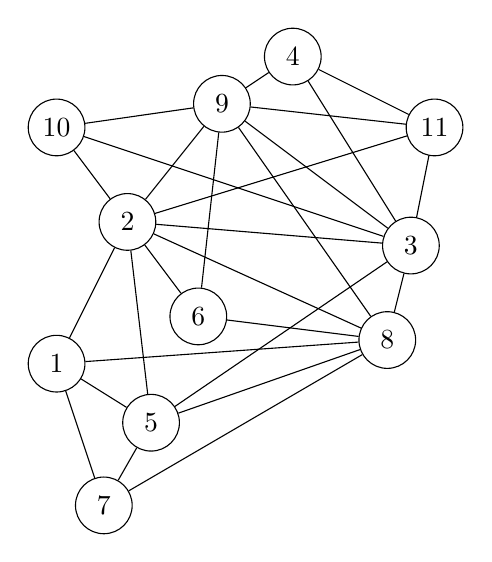
\begin{tikzpicture}
          [scale=.6,auto=left,every node/.style={draw, circle, inner sep = 0pt, minimum width = 0.72cm}]
        \node (n10) at (1,9) {10};
        \node (n2) at (2.5,7) {2};
        \node (n1) at (1,4) {1};
        \node (n5) at (3,2.75) {5};
        \node (n7) at (2,1) {7};
        \node (n9) at (4.5,9.5) {9};
        \node (n6) at (4,5) {6};
        \node (n4) at (6,10.5) {4};
        \node (n3) at (8.5,6.5) {3};
        \node (n8) at (8,4.5) {8};
        \node (n11) at (9,9) {11};

        \foreach \from/\to in {n1/n2, n1/n5, n1/n7, n1/n8, n2/n3, n2/n5, n2/n6, n2/n8, n2/n9, n2/n10, n2/n11, n3/n4, n3/n5, n3/n8, n3/n9, n3/n10, n3/n11, n4/n9, n4/n11, n5/n7, n5/n8, n6/n8, n6/n9, n7/n8, n8/n9, n9/n10, n9/n11}
          \draw (\from) edge (\to);
      \end{tikzpicture}

      (a)
    \end{minipage}\begin{minipage}{0.5\textwidth}
      \centering
      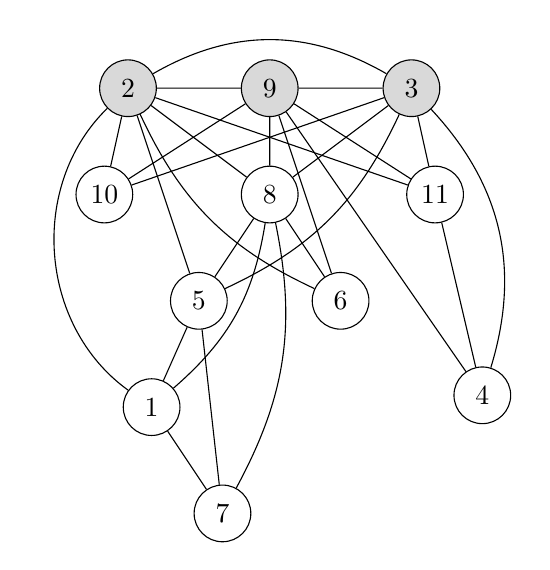
\begin{tikzpicture}
          [scale=.6,auto=left,every node/.style={draw, circle, inner sep = 0pt, minimum width = 0.72cm}]
        \node (n10) at (1,8.25) {10};
        \node[fill=gray!30] (n2) at (1.5,10.5) {2};
        \node (n1) at (2,3.75) {1};
        \node (n5) at (3,6) {5};
        \node (n7) at (3.5,1.5) {7};
        \node[fill=gray!30] (n9) at (4.5,10.5) {9};
        \node (n6) at (6,6) {6};
        \node (n4) at (9,4) {4};
        \node[fill=gray!30] (n3) at (7.5,10.5) {3};
        \node (n8) at (4.5,8.25) {8};
        \node (n11) at (8,8.25) {11};

        \foreach \from/\to in {n1/n5, n1/n7, n2/n5, n2/n8, n2/n9, n2/n10, n2/n11, n3/n8, n3/n9, n3/n10, n3/n11, n4/n9, n4/n11, n5/n7, n5/n8, n6/n8, n6/n9, n8/n9, n9/n10, n9/n11}
          \draw (\from) edge (\to);

        \draw (n1) edge [bend right=20] (n8);
        \draw (n1) edge [bend left=50] (n2);
        \draw (n2) edge [bend left] (n3);
        \draw (n2) edge [bend right=20] (n6);
        \draw (n3) edge [bend left] (n4);
        \draw (n3) edge [bend left=20] (n5);
        \draw (n7) edge [bend right=20] (n8);
      \end{tikzpicture}

      (b)
    \end{minipage}

    \caption{
      \textbf{(a)} Uma \emph{$3$-tree} $T_3$ com 11 vértices.
      \textbf{(b)} A mesma \emph{$3$-tree} ($T_3$) enraizada no clique $\{2, 3, 9\}$.
    }
    \label{fig:rootedktree}
  \end{figure}
\end{definition}

\begin{definition}[\emph{partial $k$-tree}]
  \cite{bodlaender} Um subgrafo de uma \emph{$k$-tree} é chamado de \emph{partial $k$-tree}. Um grafo é uma \emph{partial $k$-tree} se e só se ele tem \emph{treewidth} menor ou igual a $k$.
\end{definition}

\section{Probabilidade}

A escrever. \cite{koller} % TODO

\section{Redes bayesianas}

A escrever. \cite{koller} % TODO

% TODO: onde falar de aprendizagem e inferência?
